\section{Cel i zakres ćwiczenia}
\label{sec:cel}

Wykonanie pomiarów hałasu w środowisku pochodzącego od Stacji Gazowej NR. 08/3159, zlokalizowanej na terenach zielonych, przy skrzyżowaniu ulic Oleandry i Romana Ingardena. 

Pomiary przeprowadzono metodą próbkowania, zgodnie
z metodyką referencyjną przedstawioną w instrukcji
laboratoryjnej.

Zakres opracowania obejmuje charakterystykę zbadanego obiektu oraz otoczenia, dokumentacje pomiarowych stanowisk, przedstawienie uzyskanych wyników i ocenę poziomu hałasu.

% \begin{figure}[H]
%     \centering
%     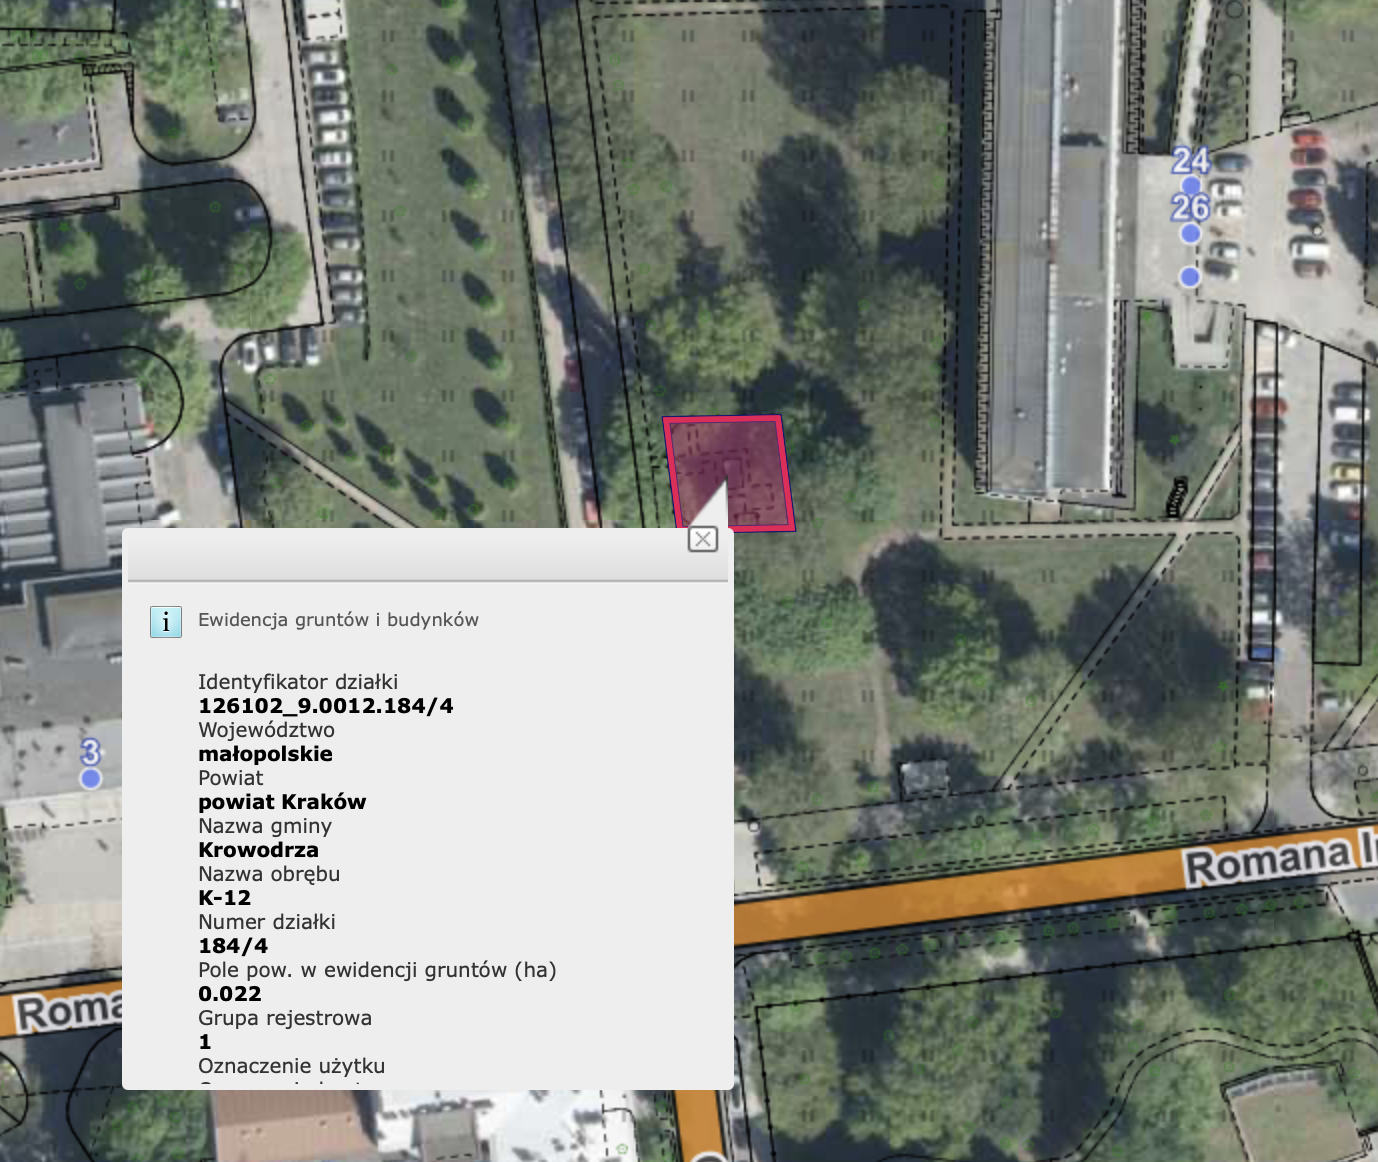
\includegraphics[
%         width=0.7\linewidth
%     ]{cwiczenia/01-pomiar-poziomu-cisnienia/figures/lokalizacja_stacji.png}
%     \caption{Lokalizacja stacji gazowej z geoportal.gov.pl}
%     \label{fig:lokalizacja}
% \end{figure}